\section{Algorithm Converter}

There are several efforts to extract formal ECMAScript semantics for static analysis
or verifications of JavaScript programs~\cite{???}. However, existing researches
manually extract the semantics and only target specific version of
EMCAScript specifications, mostly ECMAScript 5.1.
It is the critical problem to treat real-world JavaScript programs
because ECMAScript specifications are annually updated after 2015.

To alleviate such problems, we propose to automatically extract semantics from
ECMAScript specifications. Their semantics are provided as \textit{abstract algorithms}
written in structural natural langauges. Our main idea is to convert such algorithms
into our small core languages. The algorithm converter consits of multiple rules
for each layer. Moreover, we provide \textit{rule generation assistant}.
It diagnoses root causes of failed conversions and suggests
that which layer of rules should be extended for them.

\subsection{Abstract Algorithms}

Abstract algorithms in ECMAScript specifications are written in structural
natural languages. For example, Figure~\ref{fig:to-primitive} describes
the \( \code{ToPrimitive} \) abstract algorithm. It takes two parameters
\( \code{input} \) and \( \code{PreferredType} \) and evaluates its body
with given arguments. Its body consits of multiple steps and each step could
have multiple sub-steps as well. While it is not easy to infer exact meaning
of natural languages, fortunately, there is additional HTML tags are attached
into several tokens in abstract algorithms. For example, all the paramters
and newly defined local identifiers have \( \code{<var>} \) tags.
We utilize such information to construct more precise semantics.
The following table describes the list of HTML tags we utilize
and their meaning:

\[
  \begin{array}{c|l}

    \text{tags} & \text{descriptions}\\\hline\hline
    \code{<code>} & \text{ECMAScript codes}\\\hline
    \code{<emu-const>} & \text{constant values}\\\hline
    \code{<emu-grammar>} & \text{productions}\\\hline
    \code{<emu-nt>} & \text{non-terminal syntax}\\\hline
    \code{<emu-val>} & \text{values}\\\hline
    \code{<ol>} & \text{ordered sub-steps}\\\hline
    \code{<sup>} & \text{superscripts}\\\hline
    \code{<ul>} & \text{unordered sub-steps}\\\hline
    \code{<var>} & \text{variables}\\\hline
  \end{array}
\]

\subsection{Layered Rule-based Conversions}

We convert abstract algorithms 

\subsubsection{Layered Rules}

% 각각의 layer를 어떻게 나누었나를 설명
% 가장 많이 match하는 경우? 중복되는 경우?
% 예시 보여주기

\subsubsection{Core Language for ECMAScript}

% core의 특성을 정리해서 보여주기 formal?
% data와 type을 어떤 식으로 다루는 지 알려주기
% 예시 보여주기

\subsection{Rule Generation Assistant}

% 각 module들 설명하기














\inred{
\subsection{Core language}
실행 가능한 specification을 만들기 위한 langauge.
algorithm들의 공통된 행동을 실행할 수 있게 잘 설계함
ex) let X be ... => let X = ...

\subsubsection{다른 rewriting system 또는 compiler와 다른 점}
특징으로는 Parser에서 만들어진 AST를 하나의 값으로 들고 다니면서 관련 함수를 호출하거나 subAST를 가져올수 있게 만들어짐. 이는 Syntax function 실행을 위해선데 이후 initial state organization에서 설명 
또한 ES specification에서 공통적으로 동작하는 복잡한 연산을 expression으로 지원함, 특히 문서에 covered by에 있는 것처럼 AST Value를 Goal symbol로 다시 parse해야 하는 경우도 있고, eval이나 Class creation 관련 함수에서처럼 string을 AST로 parse해야하는 경우도 있음. 그런 경우를 parse-syntax 를 넣어서 처리할 수 있게
해줌.

\subsection{함수의 의미 번역 (algorithm => Function)}
Function은 parameter와 body로 나뉨
\subsubsection{parameter extraction} : HTML에 써있음 + 여러 특별한 말들 (with parameter * )
Builtin function의 경우 specification 내에서 implicit하게 전해지는 parameter들이 있는데, (thisValue, newTarget) 이것을
core에서 모두 명시적으로 받게 (지금은 javascript 단에서) 자동으로 고쳐준다.

\subsubsection{body extraction ( AlgoCompiler )} : 이부분이 Human resource 많이 들어감
여기서 rule에 따라 step을 만들어줌
나눌 수도 있을 것 같은데 지금은 일단 instruction, expression, condition, type, value, reference을 나타내는 position을 분리하고 거기에 맞춰서 case별로 parser를 짬
근데 똑같은 의미도 여러 다른 말로 표현하기 떄문에 지금은 모든 경우를 하나씩 써놓음
또 같은 말도 context에 따라 의미가 다른 경우가 있음 (Return할때), 지금은 알고리즘의 종류에만 dependent하므로 알고리즘에 flag를 둬서 구분

간단하지 않은 알고리즘의 경우는 1) core 내에서 표현될 수 있는 경우 Function을 만들어 모델링하거나 
2) 지원하지 않는 경우가 있다


\begin{itemize}
  \item Formal definition of Core language
    \begin{itemize}
      \item Syntax
      \item Semantics
    \end{itemize}
  \item Abstract algorithms
    \begin{itemize}
      \item syntax-directed / internal method
      \item Converted into Core
    \end{itemize}
\end{itemize}
}

\begin{figure}
  \centering
  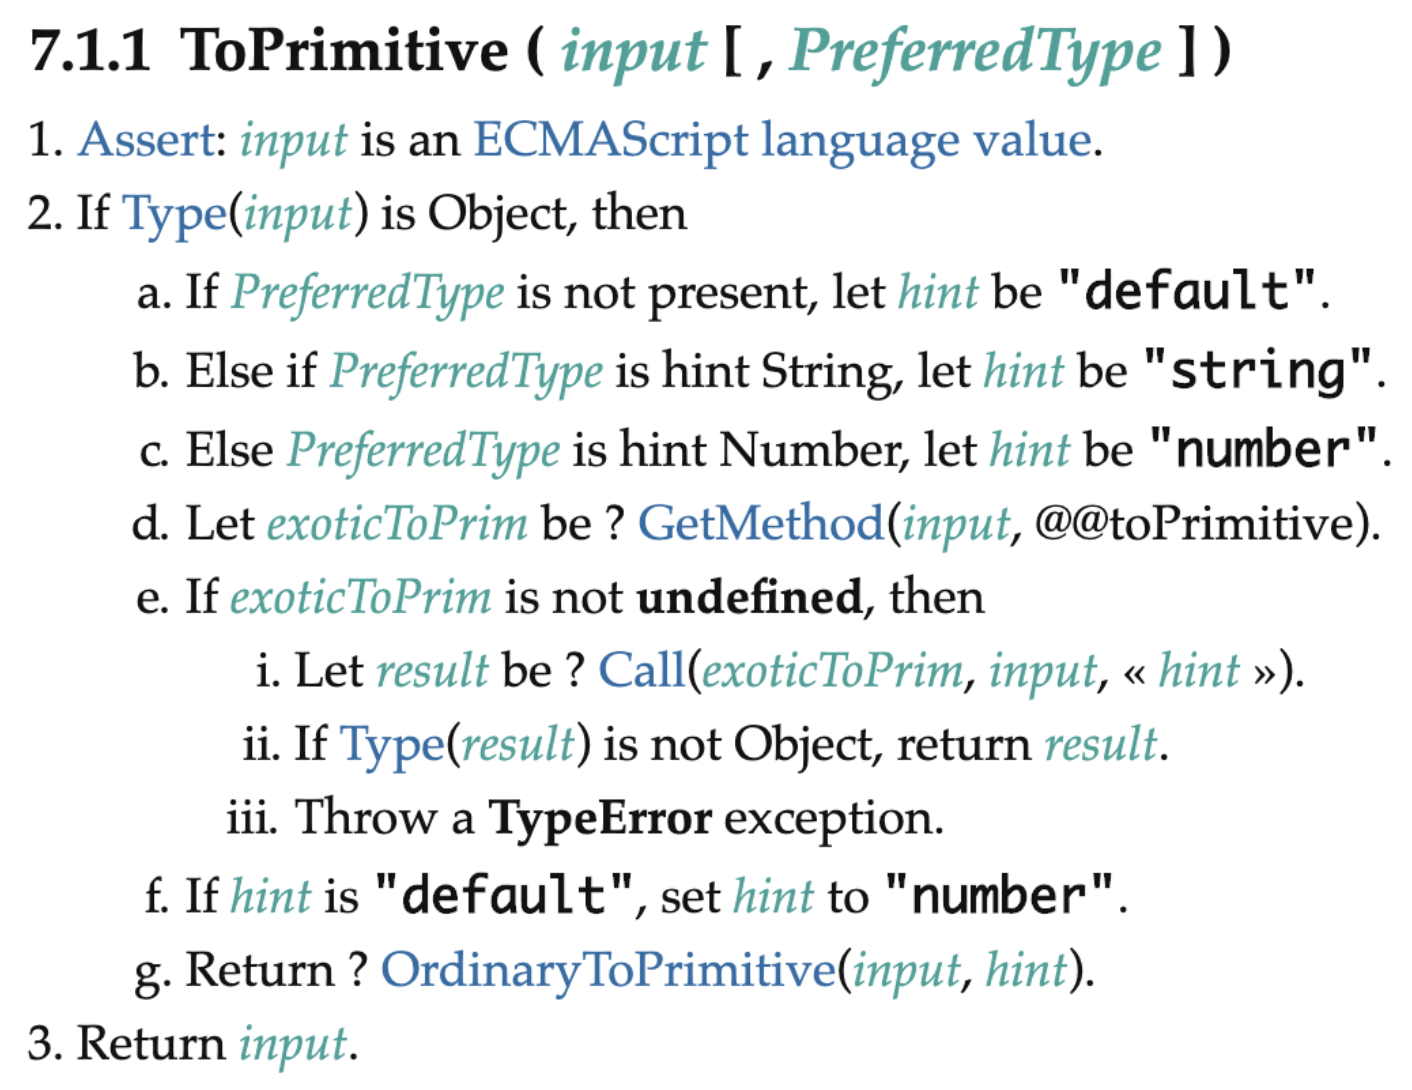
\includegraphics[height=18em]{img/to_primitive.png}
  \begin{lstlisting}[style=myCorestyle]
"ToPrimitive" (input, PreferredType) => {
  if (= (Type input) "Object") {
    if (= PreferredType absent) let hint = "default"
    else if (= PreferredType "String") let hint = "string"
    else let hint = "number"
    let exoticToPrim = ? (GetMethod input SYMBOL_toPrimitive)
    if (! (= exoticToPrim undefined)) {
      let result = ? (Call exoticToPrim input (new [hint]))
      if (! (= (Type result) "Object")) return result
      return (Throw INTRINSIC_TypeErrorPrototype)
    }
    if (= hint "default") hint = "number"
    return ? (OrdinaryToPrimitive input hint)
  }
  return input
}
  \end{lstlisting}
  \caption{\( \code{ToPrimitive} \) abstract algorithms}
  \label{fig:to-primitive}
\end{figure}

% HTML tag based token / structure 그대로 살림
% Parameter를 뽑는 방법들
% Context dependent한 return과 함수가 아닌 macro에 해당하는 returnifabrupt등을 설명
